\subsection{Automation}
\label{sec:automation}

\textbf{Purpose}: Performing growth-, maintenance-, and data-related tasks autonomously, on the basis of both schedule and necessity, to:

\begin{itemize}
    \item Reduce crew maintenance time;
    \item Improve consistency of products;
    \item Eliminate safety risks;
    \item Enable local and remote monitoring and configuration of the system;
    \item Maintain the homogeneity of the internal environment;
    \item Enable simultaneous control over all parameters.
\end{itemize}

\textbf{Function}:
\begin{itemize}
    \item \textbf{Inputs}: Subsystem data (sensor readings, status), environment program, user input (local and remote)
    \item \textbf{Outputs}: Subsystem control signals, local and remote messaging and telemetry/logging, environment data, timelapse photo set
\end{itemize}

\textbf{Method}:
\begin{enumerate}
    \item \textit{Setup}:
    \begin{enumerate}
        \item Power is connected and system is booted;
        \item System configuration is set (e.g. network, time, authentication, etc.);
        \item Program is selected by user;
    \end{enumerate}
    \item \textit{Testing}:
    \begin{itemize}
        \item Power-on Self-Test (POST) passes (i.e. all hardware is online and communicating as expected);
        \item Subsystems enact environment program in response to subsystem data;
        \item Camera capture functions as intended;
        \item Local and remote monitoring and configuration functions as intended.
    \end{itemize}
    \item \textit{Process}:
    \begin{enumerate}
        \item Checks operating preconditions (self-POST and subsystem tests);
        \item \textbf{Environment Control Loop}:
        \begin{enumerate}
            \item \textit{Sense}: Receives, stores, and logs data about current environment and system states;
            \item \textit{Plan}: Compares current environment state to environment program state and determines control action "plan" to reach desired state;
            \item \textit{Act}: Controls subsystem operations in order to enact the plan;
        \end{enumerate}
        \item Captures photos at regular intervals and stores them in a timelapse photo set;
        \item Notifies local and remote users of maintenance requirements (i.e. non-automated input/output management, refills, repairs, etc.), diagnostic information (i.e. state, errors and failures), and end-of-program/harvest/replanting times.
    \end{enumerate}
    \item \textit{Shutdown} (either manual or end-of-program):
    \begin{enumerate}
        \item Shut down all subsystem operations;
        \item Power down.
    \end{enumerate}
\end{enumerate}

\clearpage

\textbf{Features}:

A dual-system implementation was chosen to allow for discrete management of high-level functionality (camera capture, networking functionality, local storage, complex calculations, etc.) and low-level functionality (hardware-level communications i.e. sensor reading, actuator control) with a constant two-way stream of shared data.

\begin{itemize}
    \item \textit{Computer} \cite{raspberrypi}: Manages data collection, batch storage, analysis, and transmission/receiving, as well as planning/calculations for subsystem control. Includes internal clock (for program, notification), network connection (for data transmission, notification), photo capture, and non-volatile storage (for data/photos). Sends subsystem control instructions to the microcontroller.
    \item \textit{Microcontroller} \cite{arduino}: Manages subsystem sensor/actuator states and communications (on/off, sensor readings, actuator control). Streams collected sensor readings to the computer.
    \item \textit{Program}: Set of actuated instructions (e.g. lights on) and control targets (e.g. hold air temperature at 22°C) to enact at specific points in the growth cycle, as well as config data;
    \item \textit{Camera Capture \& Plant Phenotype Metric Extraction}: Top-down and side-view cameras \cite{camera}, captured under standard lighting at regular intervals throughout the course of the growth cycle. For live feed transmission to users (local and remote), as well as plant phenotype metric extraction extraction via computer vision and machine learning for yield and diagnostic analysis. Potentially relevant plant phenotype metrics include (but are not limited to):
    \begin{itemize}
        \item Leaf health indicators (i.e. leaf tip burn, leaf curl, chlorosis);
        \item Leaf count, size distribution;
        \item Leaf density;
        \item Canopy dimensions/surface area;
        \item Plant height;
        \item Fruit/harvest body size, ripeness;
    \end{itemize}
    \item \textit{Environment Data}: Record the environment's current state. Covers each \textit{control system} environment parameter (e.g. included in a feedback loop). Control system environment parameters include:
    \begin{itemize}
        \item Leaf-zone temperature (see \ref{sec:airthermoregulation});
        \item Leaf-zone humidity (see \ref{sec:humidityregulation});
        \item Root-zone temperature (see \ref{sec:aeroponics});
        \item Gas concentrations (see \ref{sec:gas});
    \end{itemize}
    \item \textit{Subsystem Control}: Induces change in environment parameters. Covers both \textit{control system} and \textit{actuated instruction} environment parameters. Actuated instruction environment parameters include:
    \begin{itemize}
        \item Lighting (see \ref{sec:lighting});
        \item Water delivery (see \ref{sec:aeroponics});
        \item Plant nutrient delivery (see \ref{sec:aeroponics});
        \item Water pH (see \ref{sec:aeroponics});
        \item Air circulation rate (see \ref{sec:airthermoregulation});
    \end{itemize}
    \item \textit{Diagnostic Systems}: Include informative sensors tracking system input availability, subsystem diagnostics, etc. as well as notification triggers.
\end{itemize}

\clearpage

\textbf{Figures}

\begin{figure}[h!]
    \centering
    \frame{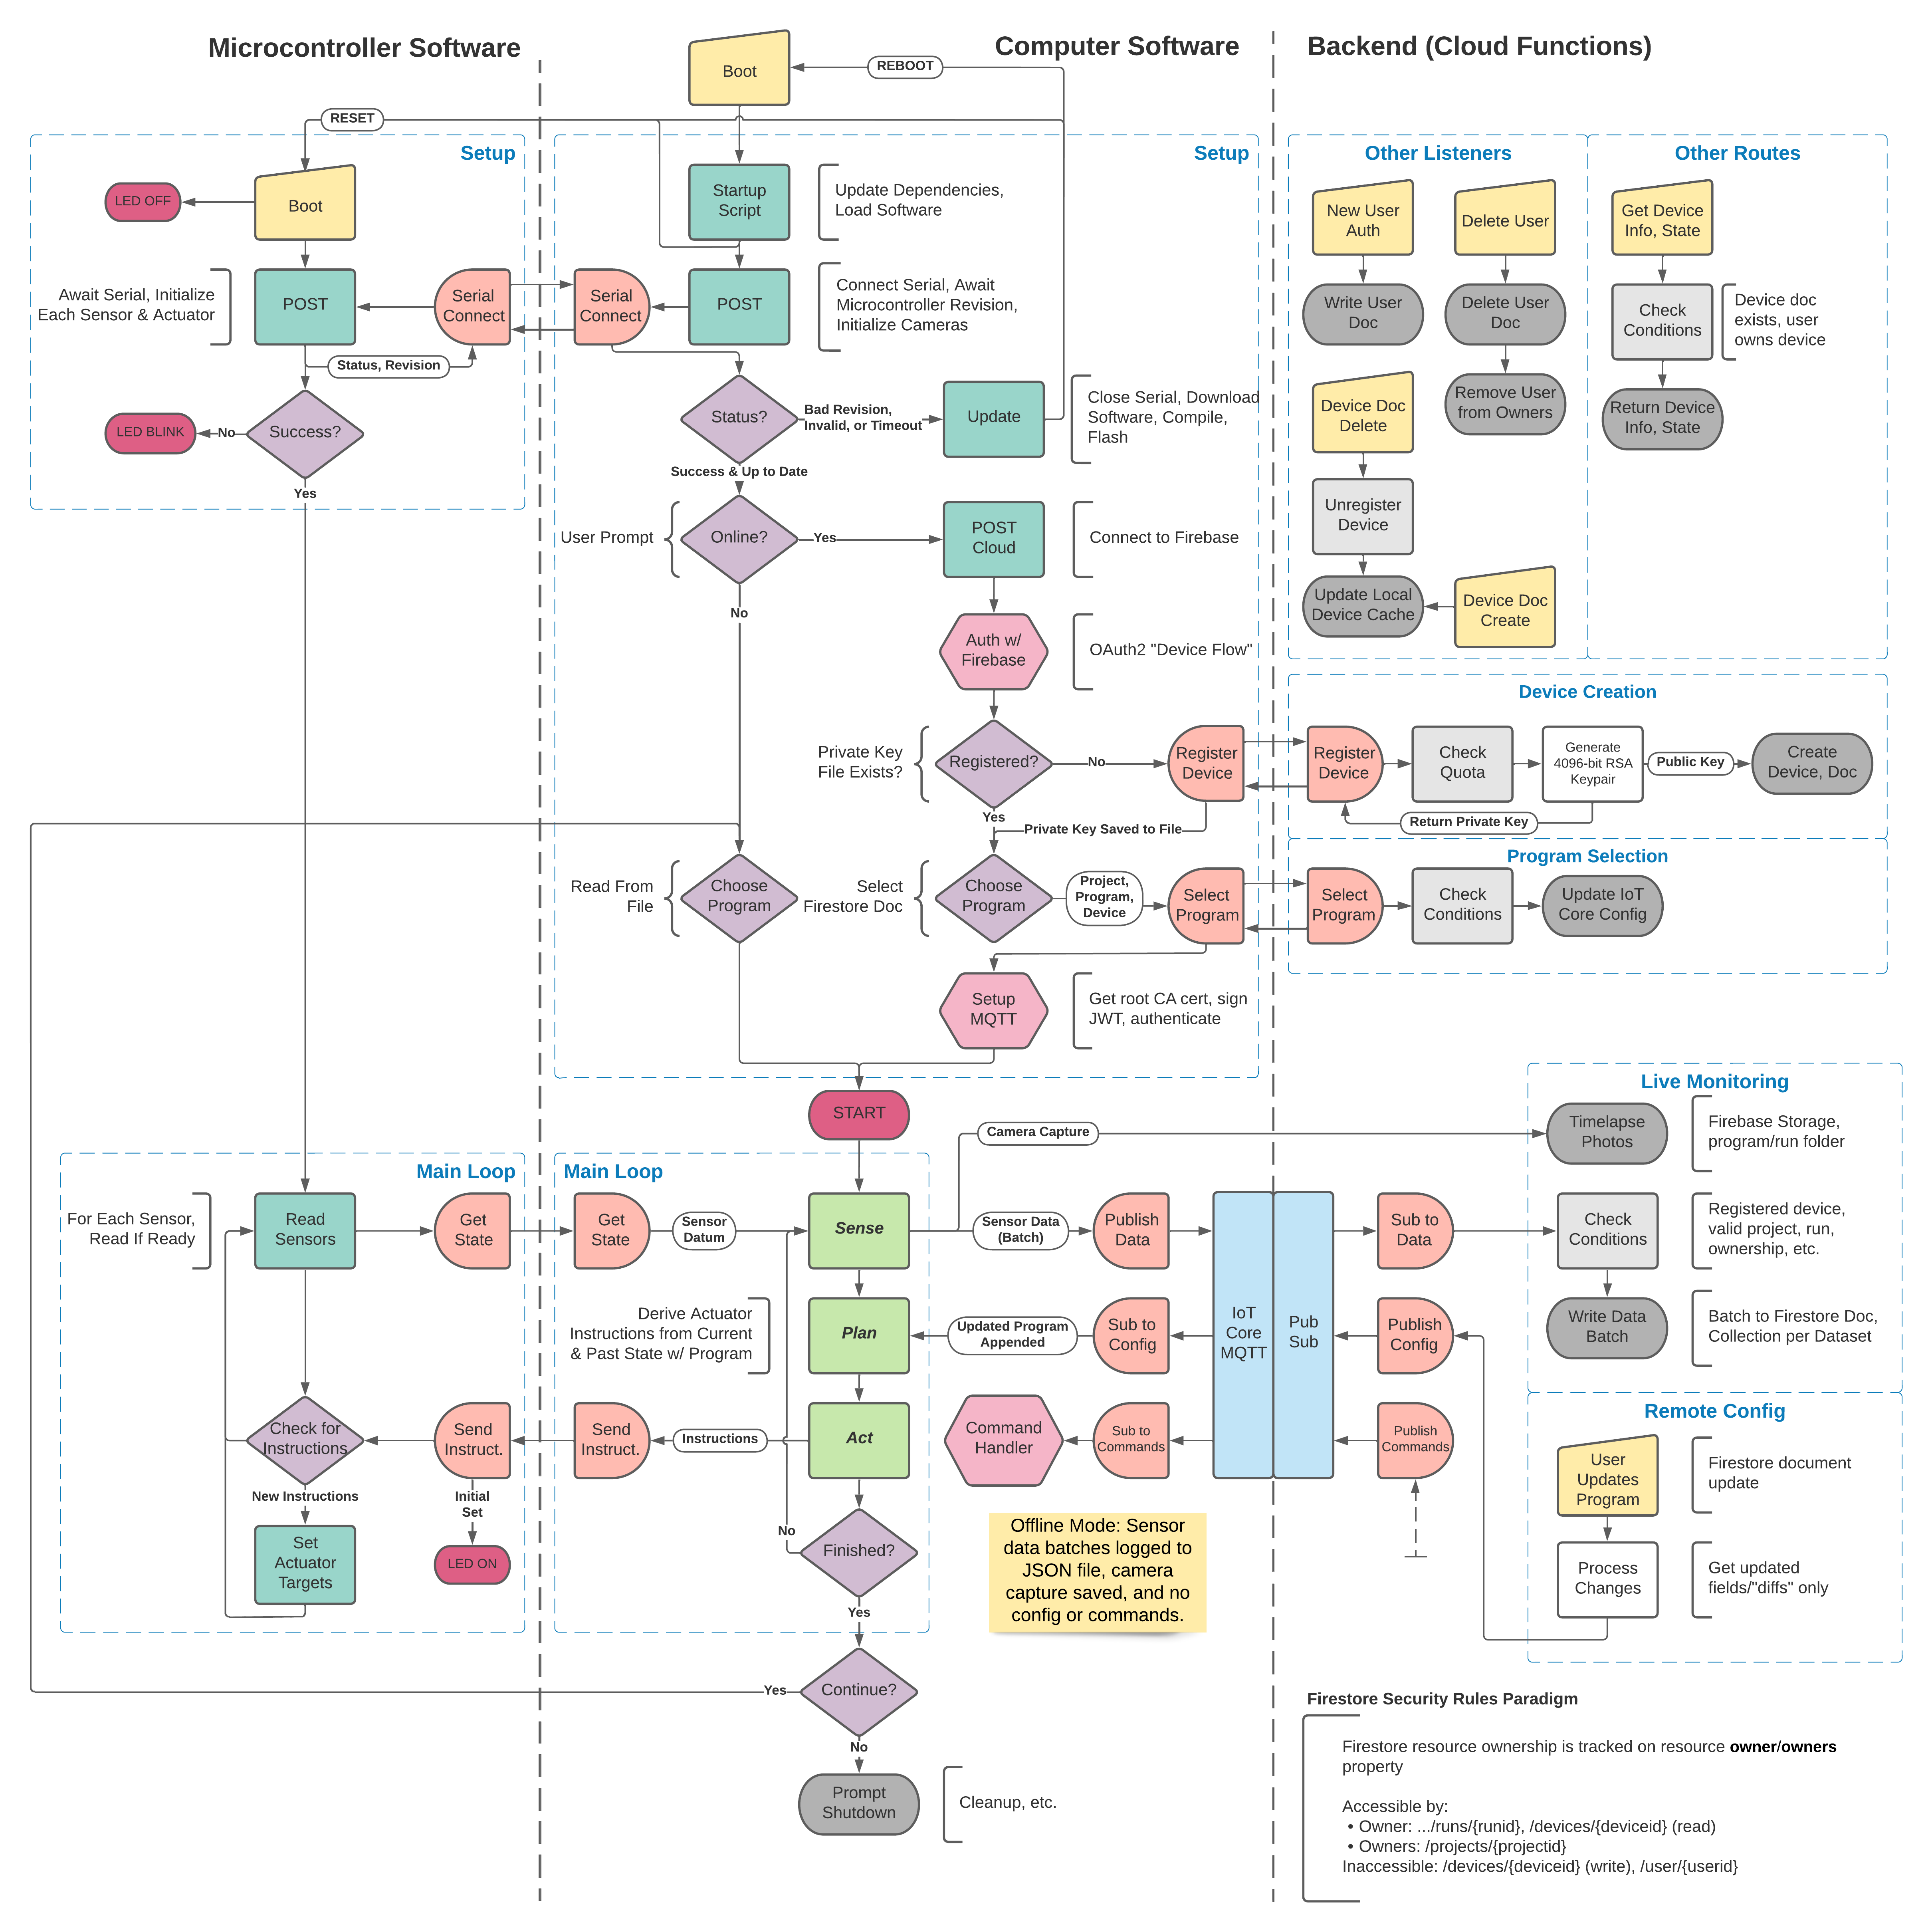
\includegraphics[width=\textwidth]{../assets/figures/automation_software.png}}
    \caption{Software control flow diagram.}
    \label{fig:automation_software}
\end{figure}

\begin{figure}[h!]
    \centering
    \frame{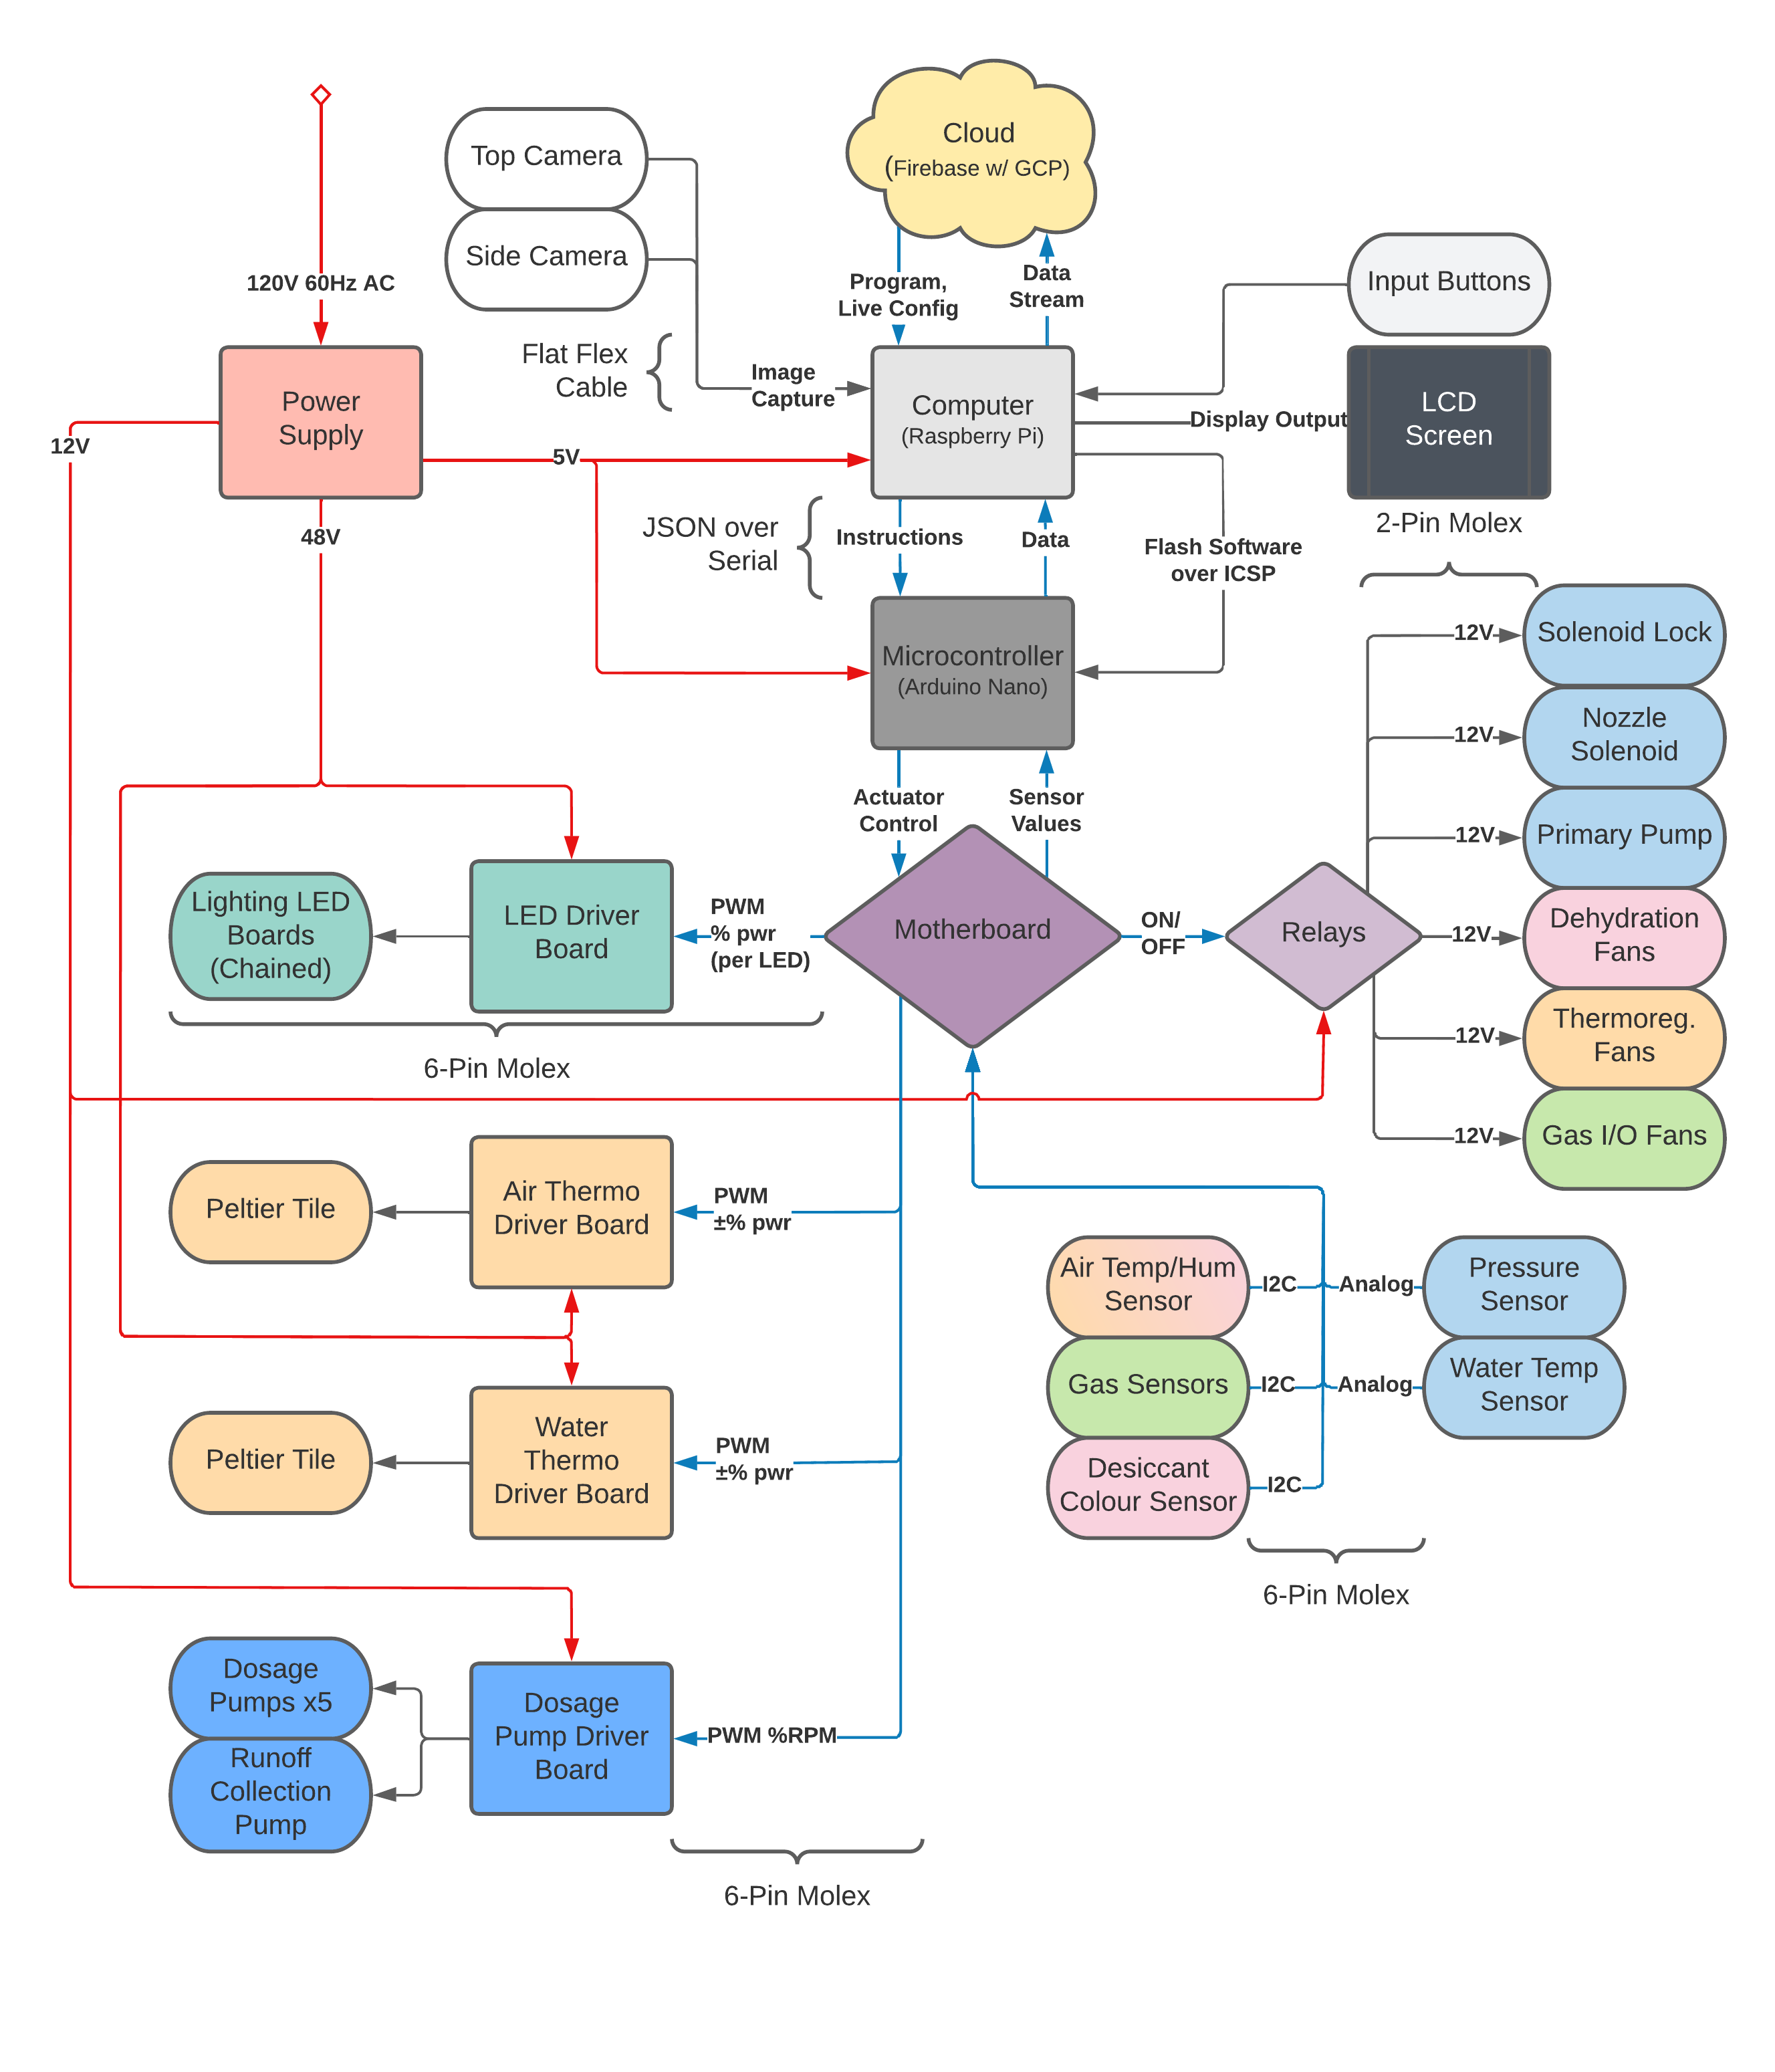
\includegraphics[width=\textwidth]{../assets/figures/automation_wiring.png}}
    \caption{System wiring diagram.}
    \label{fig:automation_wiring}
\end{figure}